
The general equation of a line can be written as :
\begin{align}
\vec{n}^T\vec{x}=c \label{aug/2/18/eq:1}  
\end{align}
where $\vec{n}$ is the normal to the line.
%
The standard basis vectors in 2D plane are given by:
\begin{align}
\vec{e_{1}} &= \myvec{1 \\ 0}\label{aug/2/18/eq:2}
\\\vec{e_{2}} &= \myvec{0 \\ 1}\label{aug/2/18/eq:3}
\end{align}
%
Let the line \eqref{aug/2/18/eq:1} cut the x and y co-ordinate axes at $\vec{A}$ and $\vec{B}$ respectively. They can be written as 
\begin{align}
\vec{A} &= \dfrac{c\vec{e_{1}}}{\vec{n}^T\vec{e_{1}}}\label{aug/2/18/eq:4}\\
\vec{B} &= \dfrac{c\vec{e_{2}}}{\vec{n}^T\vec{e_{2}}}\label{aug/2/18/eq:5}
\end{align}
%
It is given that the line cuts off equal intercepts on the co-ordinate axes. Hence from \eqref{aug/2/18/eq:4} and \eqref{aug/2/18/eq:5} we have
\begin{align}
\vec{n}^T\vec{e_{1}} = \vec{n}^T\vec{e_{2}}
\end{align}
%
which is equivalent to
\begin{align}
\vec{n}^T(\vec{e_{1}}-\vec{e_{2}}) &= 0\\
\vec{n}^T\myvec{1 \\ -1} &= 0\\
\implies \vec{n} = \myvec{1 \\ 1}\label{aug/2/18/eq:6}
\end{align}
%
Hence from \eqref{aug/2/18/eq:1} and \eqref{aug/2/18/eq:6} , the equation of the line is given by:
\begin{align}
\myvec{1 & 1}\vec{x}=c\label{aug/2/18/eq:7}
\end{align}
It is given that $\myvec{2 \\ 3}$ lies on the line. Hence from \eqref{aug/2/18/eq:7} we have:
\begin{align}
c =\myvec{1 & 1}\myvec{2 \\ 3} = 5
\end{align}
Therefore the equation of the line is
\begin{align}
\myvec{1 & 1}\vec{x}=5
\end{align}
This is illustrated in Fig.     \ref{aug/2/18/Line AB}.
\begin{figure}[!ht]
       \centering
    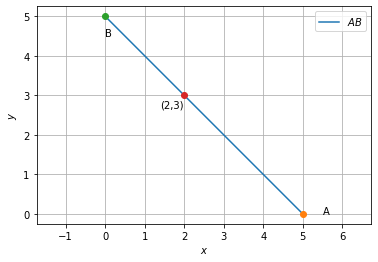
\includegraphics[width=\columnwidth] {solutions/aug/2/18/Assignment_4_Fig_1.png}
    \caption{Line $\vec{AB}$ making equal intercepts on co-ordinate axes}
    \label{aug/2/18/Line AB}
\end{figure}

